\documentclass[12pt]{article}
% Esenciales:
\usepackage[a4paper, margin=2.5cm]{geometry} % Hoja A4 con margen de 2.5cm
\usepackage{tikz,pgfplots}
\usepackage{graphicx}
\usepackage{float}

% Tipo de letra
% Arial:
\renewcommand{\familydefault}{\sfdefault}
% Comentar Arial y descomentar las siguientes para Helvetica:
% \usepackage{helvet}
% \renewcommand{\familydefault}{\sfdefault}

% Para citas bibliograficas:
\usepackage[backend=bibtex, style=numeric]{biblatex}
\addbibresource{bib/referencias.bib}

% Índice clickeable
% \usepackage[colorlinks=true, linkcolor=black]{hyperref}
\usepackage[
  colorlinks=true,
  linkcolor=black,      % Títulos, referencias internas, índice
  citecolor=black,      % Citas [1], [2], etc.
  urlcolor=blue         % Enlaces web
]{hyperref}

\usepackage[utf8]{inputenc}
\usepackage[T1]{fontenc}
\usepackage{listings}          % Para código
\usepackage{xcolor}            % Para colores


\usepackage{titlesec}   % Para modificar títulos
\usepackage{tocloft}    % Para personalizar el índice
% --- Ocultar números en títulos (pero mantener en índice) ---
\titleformat{\section}
  {\color{cyan!45!black}\normalfont\Large\bfseries}{}{0em}{}

\titleformat{\subsection}
{\color{black}\normalfont\large\bfseries}{}{0em}{}  % Sin número visible y con color
  

% --- Asegurar que el índice muestre los números ---
\renewcommand{\cftsecaftersnum}{.}       % Punto después del número (opcional)
\renewcommand{\cftsubsecaftersnum}{.}    % Ej: "1.2." en el índice       % Carga paquetes
% --- Carga colores si no están en paquetes.tex ---
% --- Paleta VSCode White/Dark ---
% Para el fondo en códigos (255 -> blanco, 0 -> negro):
\definecolor{vsBackground}{RGB}{255, 255, 255}
\definecolor{vsText}{RGB}{0, 0, 0}
\definecolor{vsKeyword}{RGB}{86, 156, 214}
\definecolor{vsComment}{RGB}{80, 153, 85}
\definecolor{vsString}{RGB}{206, 145, 120}
\definecolor{vsLineNumbers}{RGB}{100, 100, 100}

% --- Estilo común (basado en VSCode Dark) ---
\lstdefinestyle{vsDarkStyle}{
    backgroundcolor=\color{vsBackground},
    basicstyle=\ttfamily\color{vsText}\small,
    keywordstyle=\color{vsKeyword},
    commentstyle=\color{vsComment},
    stringstyle=\color{vsString},
    numberstyle=\color{vsLineNumbers},
    showstringspaces=false,
    numbers=left,
    frame=none,
    breaklines=true,
    tabsize=4,
    xleftmargin=15pt,
    escapeinside={(*@}{@*)},
    literate= % Caracteres especiales (¡, ñ, etc.)
      {á}{{\'a}}1 {é}{{\'e}}1 {í}{{\'i}}1 {ó}{{\'o}}1 {ú}{{\'u}}1
      {Á}{{\'A}}1 {É}{{\'E}}1 {Í}{{\'I}}1 {Ó}{{\'O}}1 {Ú}{{\'U}}1
      {ñ}{{\~n}}1 {Ñ}{{\~N}}1
      {¡}{{!`}}1  {¿}{{?`}}1
      {"}{{\textquotedbl}}1
      {°}{{\textdegree}}1
      {|}{{\textbar}}1
      {~}{{\textasciitilde}}1,
}


% --- Lenguajes ---

\lstdefinelanguage{C}{
    style=vsDarkStyle,
    morekeywords={int, float, double, char, bool, true, false, NULL, sizeof, const, struct, typedef},
    morecomment=[l]{//},       % Comentarios de una línea
    morecomment=[s]{/*}{*/},   % Comentarios multilínea
    morestring=[b]{"},         % Strings entre comillas
    sensitive=true,            % Distingue mayúsculas/minúsculas
}

\lstdefinelanguage{JavaScript}{
    style=vsDarkStyle,
    morekeywords={let, const, var, function, if, else, for, while, return, class, import, export, console, async, await},
    morecomment=[l]{//},
    morecomment=[s]{/*}{*/},
    morestring=[b]{"},         % Strings con "
    morestring=[b]{'},         % Strings con '
    sensitive=true,
}

\lstdefinelanguage{Python}{
    style=vsDarkStyle,
    morekeywords={def, class, lambda, with, yield, try, except, import, from, as, self, None, True, False},
    morecomment=[l]{\#},       % Comentarios con #
    morestring=[b]{"},         % Strings con "
    morestring=[b]{'},         % Strings con '
    morestring=[s]{"""}{"""},  % Docstrings
    sensitive=true,
}

\lstdefinelanguage{MATLAB}{
    style=vsDarkStyle,
    morekeywords={function, end, if, else, elseif, for, while, switch, case, otherwise, try, catch, classdef, properties, methods},
    morecomment=[l]{\%},       % Comentarios con %
    morestring=[b]{'},         % Strings con '
    sensitive=false,           % MATLAB no distingue mayúsculas/minúsculas en keywords
} % Carga configs de código
\pgfplotsset{compat=1.18} % Set pgfplots compatibility mode

% ===== Variables editables =====
\newcommand{\materia}{Nombre de la materia}       % Nombre de la materia
\newcommand{\titulo}{PRÁCTICA 2: MODELOS DE PROPAGACIÓN } % Título del trabajo
\newcommand{\profesor}{Noé Torres Cruz}            % Nombre del profesor
\newcommand{\alumno}{\\ Guillén González Carlos Jael}             % Nombre del alumno
\newcommand{\alumnodos}{Rodriguez Gallegos Sara}             % Nombre del alumno
\newcommand{\grupo}{2TM6}
\newcommand{\fecha}{23-06-25}                  % Fecha (puede ser manual: "1 de mayo de 2024")


\begin{document}
% portada_informe.tex
\begin{titlepage}
    % --- Logos en tabla ---
    \noindent
    \begin{tabular}{@{} p{0.5\textwidth} p{0.5\textwidth} @{}}
        
\includegraphics[width=0.8\linewidth]{./img/logo-ipn.png} &
        \hfill 
\includegraphics[width=0.6\linewidth]{./img/logo-upiita.png} \\
    \end{tabular}


    \centering
    \vspace*{1cm}
    {\huge \textbf{Instituto Politécnico Nacional} \par}
    {\LARGE \textbf{Unidad Profesional Interdisciplinaria de Ingeniería y Tecnologías Avanzadas} \par}
    \vspace{1.5cm}
    {\LARGE \textbf{\materia} \par} % Variable: materia
    \vspace{1cm}
    {\Huge \titulo \par}            % Variable: título
    \vspace{2cm}
    {\large \textbf{Profesor:} \profesor \par} % Variable: profesor
    {\large \textbf{Alumnos:} \alumno \par}     % Variable: alumno
    {\large \alumnodos}
    \vfill
    {\large \textbf{\grupo} \par}       % Variable: grupo
    
    {\large \fecha \par}            % Variable: fecha
\end{titlepage}

\tableofcontents
\clearpage
\section{Objetivo}

Analizar y comparar distintos modelos de propagación de señal en sistemas celulares (como el modelo de espacio libre, superficie reflejante, COST231 y lognormal) mediante la implementación de simulaciones y el análisis de datos obtenidos a partir de mediciones reales, con el fin de comprender el comportamiento de la potencia recibida en función de la distancia y las condiciones del entorno, tanto con línea de vista (LoS) como sin línea de vista (NLoS).

\section{\Large Introducción}

La propagación de ondas electromagnéticas es un aspecto fundamental en el dise\~no de redes de comunicación inalámbrica, especialmente en sistemas celulares. Los modelos de propagación permiten predecir cómo se comporta la se\~nal en diferentes condiciones ambientales, topográficas y estructurales. En esta práctica se exploran cuatro modelos fundamentales: Modelo de Espacio Libre, Superficie Reflejante, COST231-Walfish-Ikegami y Lognormal con Ensombrecimiento. Además, se aborda la detección de línea de vista (LoS), un criterio clave en la selección del modelo adecuado.

\subsection{Modelo de Espacio Libre}
Este modelo representa una condición ideal en la que no existen obstrucciones entre el transmisor y el receptor. Se basa en la ley del inverso del cuadrado y describe cómo la potencia disminuye con el cuadrado de la distancia:

\begin{equation}
L\_{fs} = 32.44 + 20\log\_{10}(d\_{km}) + 20\log\_{10}(f\_{MHz})
\end{equation}

\noindent Donde:
\begin{itemize}
\item $L\_{fs}$: Pérdida de trayectoria (dB),
\item $d\_{km}$: Distancia en kilómetros,
\item $f\_{MHz}$: Frecuencia en megahercios.
\end{itemize}

\begin{figure}[H]
\centering
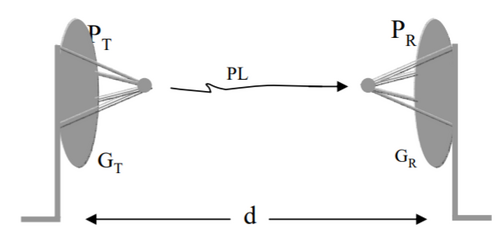
\includegraphics[width=0.5\textwidth]{./img/espaciolibre.png}
\caption{Modelo de espacio libre. La se\~nal viaja sin obstrucciones.}
\end{figure}

\subsection{Modelo de Superficie Reflejante}
Este modelo considera que la se\~nal se refleja en el suelo antes de alcanzar el receptor, generando interferencia constructiva o destructiva:

\begin{equation}
L\_{sr} = 40\log\_{10}(d\ [m]) - 20\log\_{10}(ht)(hr)
\end{equation}

\noindent Donde:
\begin{itemize}
\item $d$: Distancia en metros,
\item $ht$: Altura del transmisor,
\item $hr$: Altura del receptor.
\end{itemize}

\begin{figure}[H]
\centering
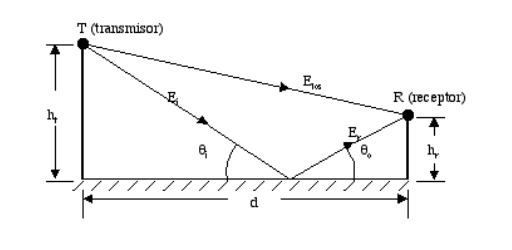
\includegraphics[width=0.5\textwidth]{./img/reflejante.png}
\caption{Modelo con reflexión en superficie terrestre.}
\end{figure}

\subsection{Modelo COST231-Walfish-Ikegami}
Este modelo se usa en entornos urbanos. Considera la influencia de edificios, calles y la geometría urbana. Se divide en pérdidas de trayectoria básica, de techo a calle y por difracción:

\begin{align}
L &= L_0 + L_{rts} + L_{msd} \\
L_0 &= 32.4 + 20\log_{10}(d_{km}) + 20\log_{10}(f_{MHz}) \\
L_{rts} &= -16.9 - 10\log_{10}(w) + 10\log_{10}(f) + 20\log_{10}(h_t - h_r) + L_{ori} \\
L_{msd} &= L_{bsh} + k_a + k_d \log_{10}(d) + k_f \log_{10}(f) - 9 \log_{10}(b)
\end{align}

\noindent Parámetros:
\begin{itemize}
\item $w$: Ancho de calle, $b$: Separación entre edificios,
\item $L_{ori}$: Pérdida por orientación, $L_{bsh}$: Pérdida techo a calle,
\item $k_a = 54$, $k_d = 18$, $k_f$: Factor de frecuencia.
\end{itemize}

\begin{figure}[H]
\centering
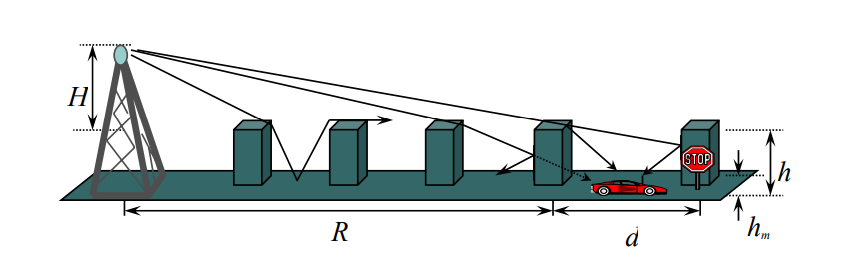
\includegraphics[width=0.5\textwidth]{./img/walfish.png}
\caption{Modelo COST231 considerando estructura urbana.}
\end{figure}

\subsection{Modelo Lognormal con ensombrecimiento}
Este modelo incorpora la variabilidad aleatoria debida a obstrucciones como edificios o árboles. La pérdida total incluye una componente aleatoria:

\begin{equation}
L\_{\log} = 10 \alpha \log\_{10}(d\_{km}) + X\_\sigma
\end{equation}

\noindent Donde:
\begin{itemize}
\item $alpha$: Exponente de pérdida,
\item $X_sigma$: Variable aleatoria normal con desviación $sigma$ (dB).
\end{itemize}

\begin{equation}
P\_{rx} = P\_{tx} + G\_{tx} + G\_{rx} - L\_{\log}
\end{equation}

\subsection{Análisis de Línea de Vista (LoS)}
La detección de LoS se basa en una evaluación geométrica entre la estación base y el receptor. Si un obstáculo (ej. edificio) intersecta la línea entre ambos puntos, se considera NLoS (Non-Line-of-Sight), lo cual modifica el modelo de propagación.

La correcta identificación de la condición LoS permite seleccionar el modelo más adecuado y obtener predicciones más precisas sobre la potencia de la se\~nal recibida.

\clearpage

\section{\Large Desarrollo}

\begin{enumerate}
	\subsection{Obteniendo los datos.}
	\item Ubicar la Estación Base (Base Station - BS), cuya ubicación es 19.503668573568277, -99.1279845883227. Usando Google Maps o por inspección directa estimar la altura a la que se encuentran colocadas las antenas.
	      \begin{figure}[H]
		      \centering
		      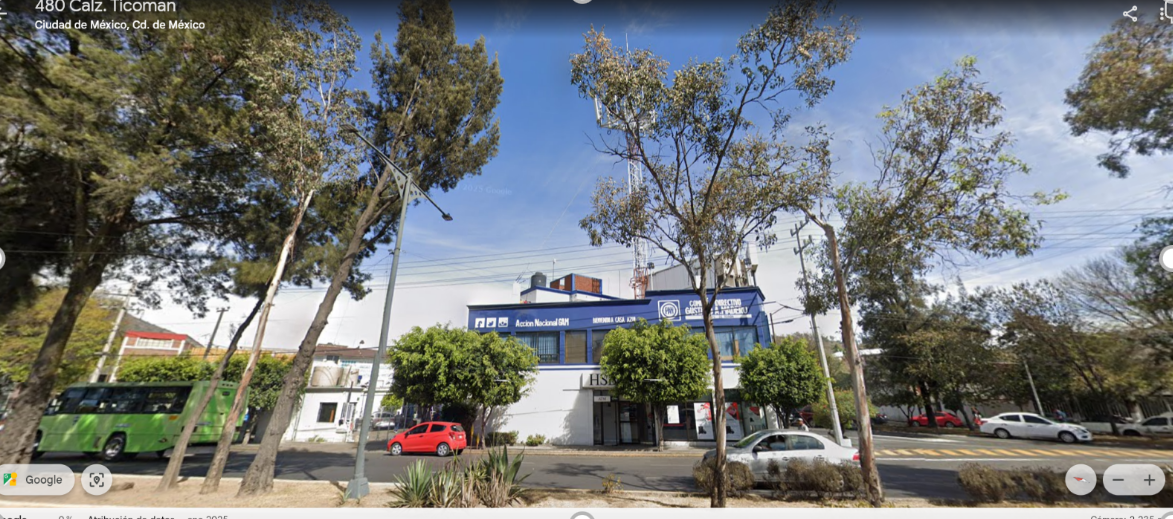
\includegraphics[width=0.9\textwidth]{./img/bs.png}
		      \caption{Imagen de la estación base en las coordenadas dadas.}
		      \label{fig:bs}
	      \end{figure}
	\item Trazar una línea recta entre la BS y la coordenada asignada y calcular la potencia recibida por cada intersección entre una calle y la línea trazada considerando los modelos espacio libre, superficie reflejante, COST231 Walfish-Ikegami y lognormal.
	      \textbf{Coordenadas: 19.508953097456004, -99.12414451054960}
	      \begin{figure}[H]
		      \centering
		      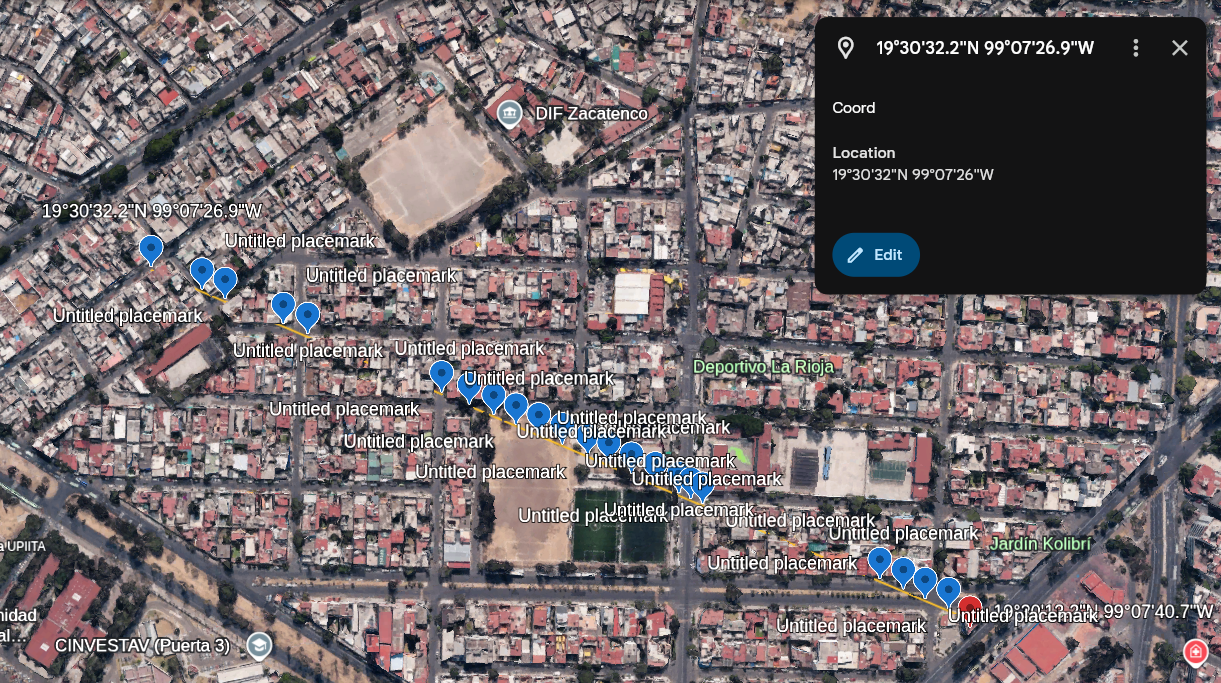
\includegraphics[width=0.9\textwidth]{./img/coordenada-dada.png} % Ajusta el ancho
		      \caption{Línea recta desde la BS hasta la coordenada asignada.}
		      \label{fig:coordenada-dada}
	      \end{figure}

	      \begin{figure}[H]
		      \centering
		      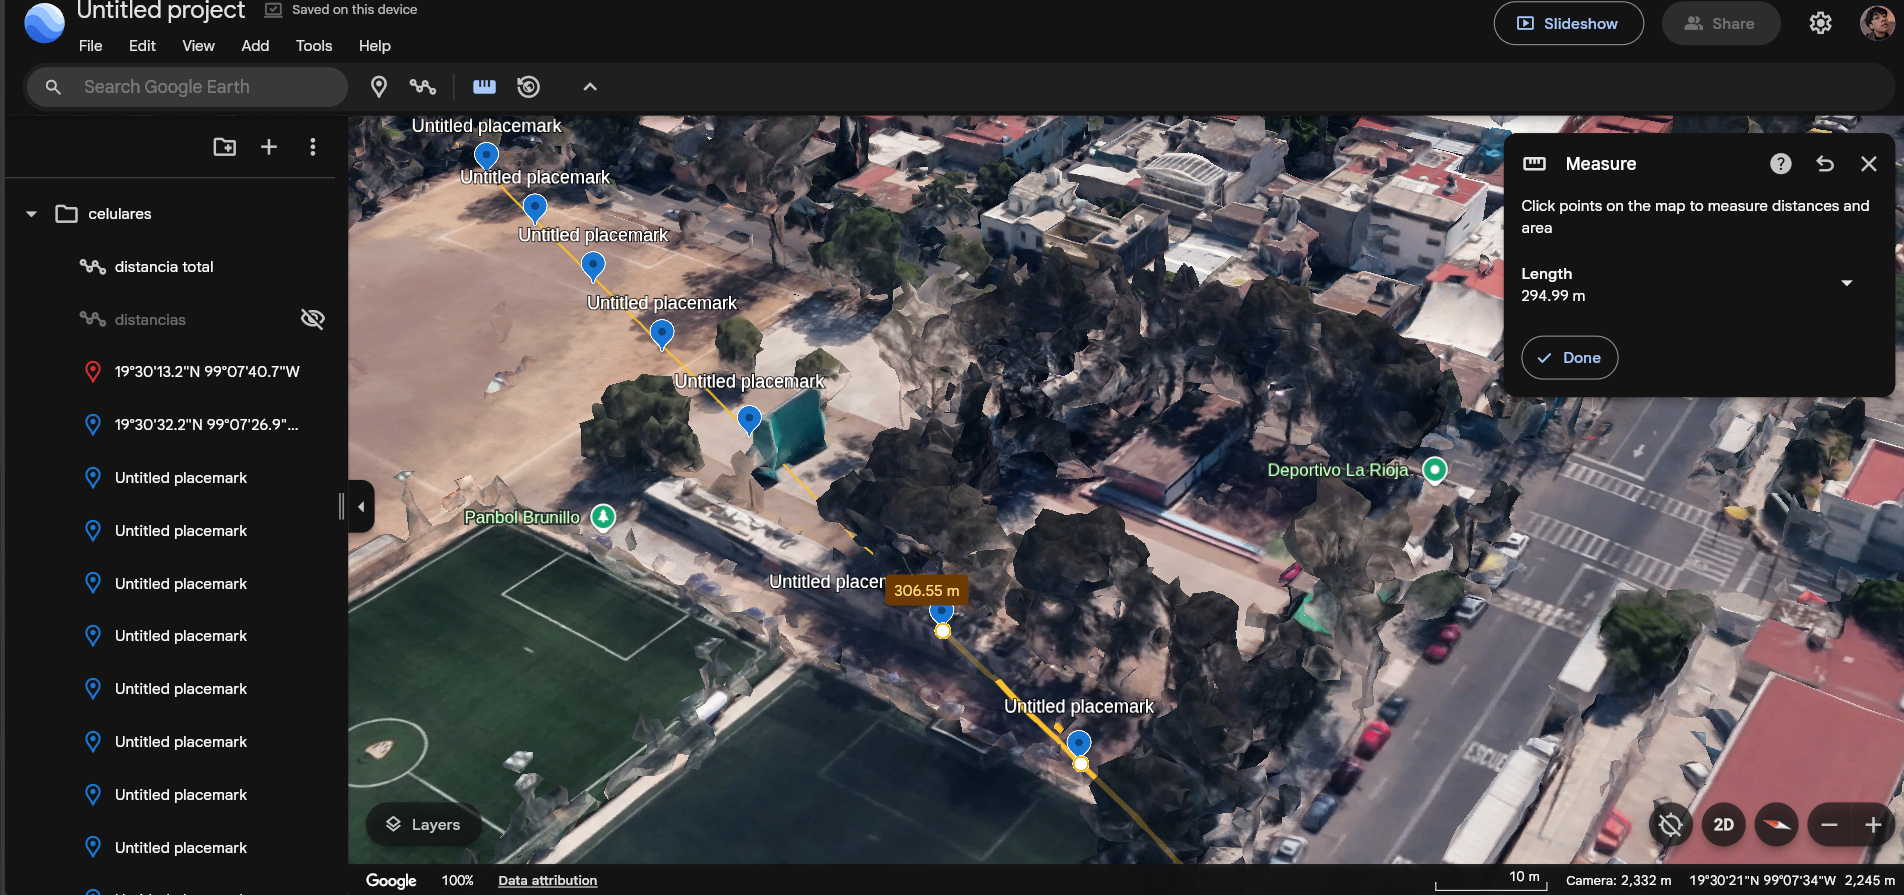
\includegraphics[width=0.9\textwidth]{./img/distancias-puntos.png} % Ajusta el ancho
		      \caption{Sacando las distancias de la BS a cada punto (aprox cada 20m en exteriores).}
		      \label{fig:distancias-puntos}
	      \end{figure}
	      \begin{figure}[H]
		      \centering
		      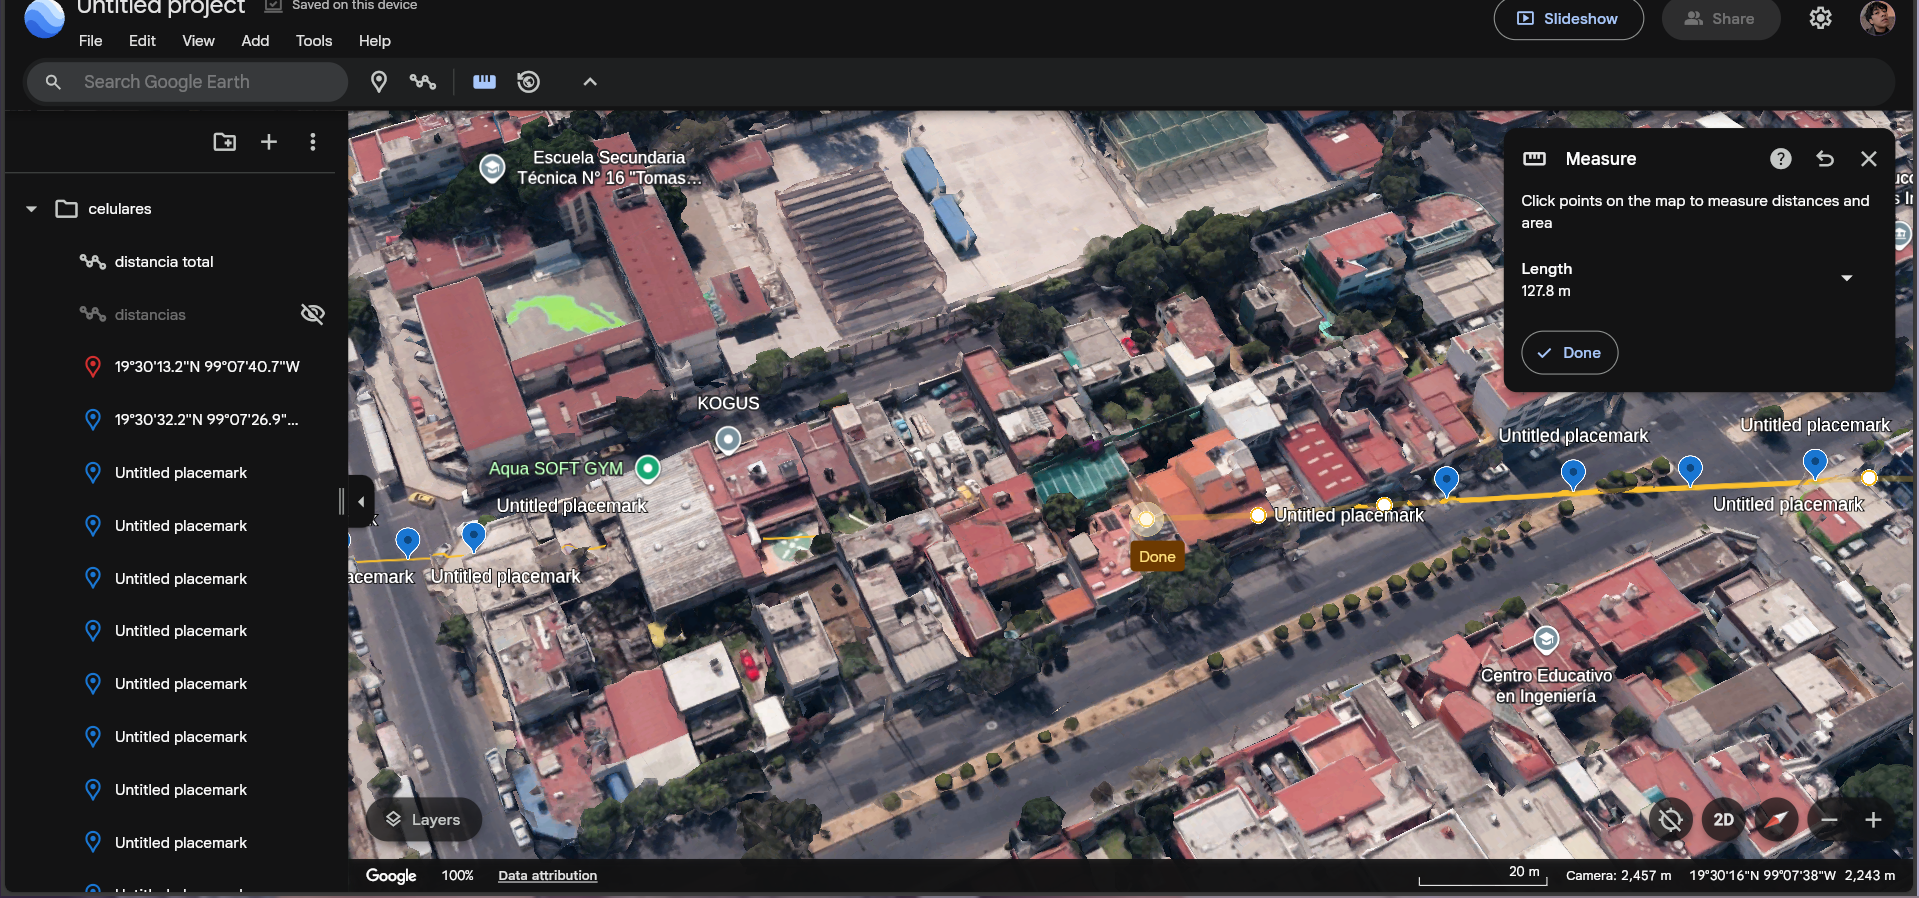
\includegraphics[width=0.9\textwidth]{./img/distancias-edificios.png} % Ajusta el ancho
		      \caption{Sacando las distancias de los edificios.}
		      \label{fig:distancias-edificios}
	      \end{figure}
	\item Considerar una frecuencia de operación de 1,935 MHz para los modelos que lo requieran. Además, considerar que la potencia de transmisión es de 10W y que las ganancias de las antenas transmisora y receptora son 9 y 3 dB, respectivamente.  
	\item Para el modelo COST231 Walfish-Ikegami realizar una tabla con los siguientes datos por cada punto analizado:  
          \begin{enumerate}
            \item Coordenadas 
            \item Distancia a la EB
            \item Si existe LOS o no 
            \item Separación promedio entre edificios, b (si aplica). 
            \item Ancho de la “calle” en la que se encuentra el móvil, w (si aplica). 
            \item Altura promedio de edificios, h (si aplica) 
            \item Ángulo de orientación, $\phi$ (si aplica).
            \item $L_0.$
            \item $L_{rts}$. (Si aplica).
            \item \item $L_{msd}$. (Si aplica).
            \item Potencia recibida (en dBm) 
          \end{enumerate}
                \begin{table}[H]
                \centering
                \begin{tabular}{|c|c|c|c|}
                    \hline
                    Coordenadas & Distancia a la EB & LOS & Potencia recibida (dBm) \\
                    \hline
                    19.50, -99.12 & 100 m & Sí & -80 \\
                    19.51, -99.13 & 120 m & No & -85 \\
                    \hline
                \end{tabular}
                \caption{Ejemplo de tabla para los puntos analizados.}
                \label{tab:ejemplo}
            \end{table}          


\end{enumerate}
\clearpage
\section{\Large Conclusión}
\clearpage
\section{\Large Anexos}
\subsection{Códigos utilizados}

\begin{lstlisting}[language=Python, caption={main.py}]
import json
import matplotlib.pyplot as plt
import math
from rich import print
from rich.table import Table
from archivos_python.determiarLOS import determinar_los
from archivos_python.walfish_ikegami import loss_los, loss_nlos
from archivos_python.logNormal import model_lognormal, generar_tabla_lognormal
from archivos_python.espacio_libre import model_free_space
from archivos_python.superficie_reflejante import model_two_ray


# Parámetros globales
FREQ_MHZ = 1935
Pt_dBm = 10 * math.log10(10) + 30  # 10 W
Gt_dB = 9
Gr_dB = 3
alpha = 2.8
sigma = 7


def main():
    # Cargar datos
    with open('datos.json', 'r') as f:
        data = json.load(f)

    h_bs = data['base_station_height']
    h_mvs = data['mobile_height']
    h_prom = data['h_prom_buildings']

    # Obtener LoS/NLoS
    los_list = determinar_los('datos.json')
    # print(los_list)
    # Modelos
    wi_results = []
    table_walfish = Table(title="[bold magenta]Resultados Modelo Walfish-Ikegami[bold magenta]")
    table_walfish.add_column("Puntos", justify="center")
    table_walfish.add_column("LOS", justify="center")
    table_walfish.add_column("ángulo", justify="center")
    table_walfish.add_column("Pérdidas [L0]", justify="center")
    table_walfish.add_column("L_rts", justify="center")
    table_walfish.add_column("L_msd", justify="center")
    table_walfish.add_column("Potencia recibida (dBm)", justify="center")

    for i, m in enumerate(data['mobiles']):
        d_metros = m['real_distance']
        d = d_metros / 1000
        phi = m['angle_deg']
        w = m['street_weight']
        b = data['prom_distance_buildings']
        angulo = m['angle_deg']
        if los_list[i]['los']:
            Lb = loss_los(d, FREQ_MHZ)
        else:
            Lb, L_rts, L_msd = loss_nlos(d, FREQ_MHZ, h_bs, h_mvs, h_prom, phi, w, b)
        Prx = Pt_dBm + Gt_dB + Gr_dB - Lb

        if(los_list[i]["los"]):
            table_walfish.add_row(f"{i+1}", "Sí", str(angulo), str(Lb), "No hay", "No hay", str(Prx))
        else: 
            table_walfish.add_row(f"{i+1}", "No", str(angulo),str(Lb), str(L_rts), str(L_msd), str(Prx))
        
        wi_results.append({'distance': d, 'Prx': Prx})

    # Lognormal
    ln_results = model_lognormal(data['mobiles'], Pt_dBm, Gt_dB, Gr_dB, alpha, sigma)
    table_lognormal = generar_tabla_lognormal(ln_results)

    # Espacio libre
    mobiles = data['mobiles']
    resultados_free_space, table_free_space = model_free_space(mobiles, FREQ_MHZ, Pt_dBm, Gt_dB, Gr_dB)
    # Modelo reflejante
    h_m = data['mobile_height']
    resultados_modelo_reflejante, table_reflejante = model_two_ray(mobiles, h_bs, h_m, FREQ_MHZ, Pt_dBm, Gt_dB, Gr_dB)

    # Imprimiendo las tablas en consola
    print(table_walfish)
    print(table_lognormal)
    print(table_free_space)
    print(table_reflejante)
    # Graficar
    distances = [r['distance'] for r in wi_results]
    Pr_wi = [r['Prx'] for r in wi_results]
    Pr_ln = [r['Pr_log'] for r in ln_results]
    Pr_free_space = [r['Prx_fspl'] for r in resultados_free_space]
    Pr_reflejante = [r['Prx_two_ray'] for r in resultados_modelo_reflejante]

    plt.figure()
    plt.plot(distances, Pr_ln, 's--', label='Lognormal')
    plt.plot(distances, Pr_reflejante, 'o--', label='Modelo reflejante')
    plt.plot(distances, Pr_free_space, 's-', label='Espacio libre')
    plt.plot(distances, Pr_wi, 'o-', label='Walfish-Ikegami')  # sin especificar color
    plt.xlabel('Distancia (m)')
    plt.ylabel('Potencia recibida (dBm)')
    plt.legend()
    plt.grid()
    plt.tight_layout()
    plt.show()

if __name__ == '__main__':
    main()
\end{lstlisting}
\clearpage
\begin{lstlisting}[language=Python, caption={walfish\_ikegami.py}]
import math

def loss_los(d, f):
    return 42.6 + 26 * math.log10(d) + 20 * math.log10(f)

import math


def lori(phi: float) -> float:
    """
    Pérdida por orientación de calle (L_ori) según COST-231 Walfish-Ikegami.
    phi: ángulo entre dirección de propagación y orientación de la calle (0°-90°)
    """
    if phi < 0 or phi > 90:
        raise ValueError("phi debe estar entre 0 y 90 grados")
    if phi < 35:
        return -10 + 0.354 * phi
    elif phi < 55:
        return 2.5 + 0.075 * (phi - 35)
    else:
        return 4.0 - 0.114 * (phi - 55)


def loss_nlos(d: float, f: float, h_bs: float, h_m: float, h_prom: float, phi: float, w: float, b: float) -> float:
    """
    Calcula las pérdidas Lb (dB) en condiciones NLoS según COST-231 Walfish-Ikegami.

    Parámetros:
    - d       : distancia real BS móvil (m)
    - f       : frecuencia (MHz)
    - h_bs    : altura de la estación base (m)
    - h_m     : altura del móvil (m)
    - h_prom  : altura promedio de edificios (m)
    - phi     : ángulo de orientación de calle (°)
    - w       : ancho de la calle (m)
    - b       : separación promedio entre edificios (m)

    Retorna:
    - Lb: pérdidas totales (dB)
    """
    # 1. Pérdida de espacio libre (L_o)
    L_o = 32.44 + 20 * math.log10(f) + 20 * math.log10(d)

    # 2. Pérdida por tejados y orientación (L_rts)
    #    w: ancho de calle
    if w <= 0:
        raise ValueError("Ancho de calle w debe ser > 0")
    delta_h = h_bs - h_prom
    term_hw = 20 * math.log10(delta_h if delta_h > 0 else 0.1)
    L_rts = (
        -16.9
        - 10 * math.log10(w)
        + 10 * math.log10(f)
        + term_hw
        + lori(phi)
    )

    # 3. Pérdida por múltiples pantallas (L_msd)
    # 3.1: L_bsh
    if h_bs > h_prom:
        L_bsh = -18 * math.log10(1 + (h_bs - h_prom))
    else:
        L_bsh = 0

    # 3.2: k_a
    if h_bs > h_prom:
        k_a = 54
    else:
        diff = h_bs - h_prom
        if d >= 500:
            k_a = 54 - 0.8 * diff
        else:
            k_a = 54 - 0.8 * diff * (d / 0.5)

    # 3.3: k_d
    if h_bs > h_prom:
        k_d = 18
    else:
        k_d = 18 - 15 * ((h_bs - h_prom) / h_prom)

    # 3.4: k_f
    k_f = -4 + 1.5 * ((f / 925) - 1)

    # 3.5: L_msd
    if b <= 0:
        raise ValueError("Separación entre edificios b debe ser > 0")
    L_msd = (
        L_bsh
        + k_a
        + k_d * math.log10(d)
        + k_f * math.log10(f)
        - 9 * math.log10(b)
    )

    # 4. Cálculo final Lb
    if (L_rts + L_msd) > 0:
        return L_o + L_rts + L_msd, L_rts, L_msd
    else:
        return L_o

\end{lstlisting}
\clearpage
\begin{lstlisting}[language=Python, caption={determinar\_LOS.py}]
import json

def check_los(h_bs, h_mvs, buildings, d_rx):
    """
    Verifica si hay línea de vista desde la BS al punto a d_rx metros.
    """
    m = (h_mvs - h_bs) / d_rx

    for b in buildings:
        x = b["x"]
        if x < d_rx:  # sólo evaluamos edificios entre BS y móvil
            h_line = h_bs + m * x
            if b["height"] > h_line:
                return False  # Obstrucción
    return True  # No hay obstrucción

def determinar_los(ruta_archivo):
    """
    Retorna booleano para decir si hay LOS o no.
    """
    with open(ruta_archivo, 'r') as f:
        data = json.load(f)

    h_bs = data["base_station_height"]
    h_mvs = data["mobile_height"]
    buildings = data["buildings"]
    resultados = []

    for movil in data["mobiles"]:
        d_rx = movil["distance_x"]
        los = check_los(h_bs, h_mvs, buildings, d_rx)
        resultados.append({
            "los": los
        })

    return resultados

# print(analizar_los_desde_json("datos.json"))
\end{lstlisting}
\clearpage
\begin{lstlisting}[language=Python, caption={espacio\_libre.py}]
import math
from rich.table import Table

def loss_free_space(d, freq_mhz):
    """
    Free-Space Path Loss (FSPL) en dB:
    FSPL = 32.44 + 20*log10(d\_km) + 20*log10(freq\_mhz)
    """
    d_km = d / 1000.0
    return 32.44 + 20 * math.log10(d_km) + 20 * math.log10(freq_mhz)


def model_free_space(mobiles, freq_mhz, Pt_dBm, Gt_dB, Gr_dB):
    """
    Calcula pérdidas FSPL y potencia recibida para cada móvil.
    Retorna lista de dicts y tabla Rich.
    """
    resultados = []
    table = Table(title="[bold cyan]Resultados Modelo Espacio Libre[/bold cyan]")
    table.add_column("Punto", justify="center")
    table.add_column("Pérdida FSPL [dB]", justify="center")
    table.add_column("Prx FSPL [dBm]", justify="center")

    for i, m in enumerate(mobiles):
        d = m['real_distance']
        Lfs = loss_free_space(d, freq_mhz)
        Prx = Pt_dBm + Gt_dB + Gr_dB - Lfs
        resultados.append({'distance': d, 'loss_fspl': Lfs, 'Prx_fspl': Prx})
        table.add_row(f"{i+1}", f"{Lfs:.2f}", f"{Prx:.2f}")

    return resultados, table

\end{lstlisting}
\clearpage
\begin{lstlisting}[language=Python, caption={log\_normal.py}]
import numpy as np

def model_lognormal(mobiles, Pt_dBm, Gt_dB, Gr_dB, alpha, sigma):
    """
    Calcula pérdidas y potencia recibida según el modelo lognormal.
    """
    dist_m = np.array([m["real_distance"] for m in mobiles])
    dist_km = dist_m / 1000
    n = len(dist_m)

    Ld_log = 10 * alpha * np.log10(dist_km)
    Xsigma = np.random.randn(n) * sigma
    Pr = Pt_dBm + Gt_dB + Gr_dB - Ld_log - Xsigma

    # Devolver lista de dicts
    return [
        {
            "distance": dist_m[i],
            "loss_d": Ld_log[i],
            "shadowing": Xsigma[i],
            "Pr_log": Pr[i]
        }
        for i in range(n)
    ]

from rich.table import Table

def generar_tabla_lognormal(resultados):
    table = Table(title="[bold magenta]Resultados Modelo Lognormal[/bold magenta]")

    table.add_column("Puntos", justify="center")
    table.add_column("Distancia (m)", justify="center")
    table.add_column("Pérdida [dB]", justify="center")
    table.add_column("Ensombrecimiento [dB]", justify="center")
    table.add_column("Potencia recibida [dBm]", justify="center")

    for index, r in enumerate(resultados):
        table.add_row(
            f"{index+1}",
            f"{r['distance']:.2f}",
            f"{r['loss_d']:.2f}",
            f"{r['shadowing']:.2f}",
            f"{r['Pr_log']:.2f}"
        )

    return table

# table = Table(title="[bold magenta]Resultados Modelo lognormal[bold magenta]")
# table.add_column("Distancia", justify="center")
# table.add_column("Pérdida [dB]", justify="center")
# table.add_column("Ensombrecimiento [dB]", justify="center")
# table.add_column("Potencia recibida [dBm]", justify="center")
\end{lstlisting}
\clearpage
\begin{lstlisting}[language=Python, caption={superficie\_reflejante.py}]
import math
from rich.table import Table

# velocidad de la luz en m/s
c = 3e8

def pr_two_ray(d, h_bs, h_m, freq_mhz, Pt_dBm, Gt_dB, Gr_dB):
    """
    Modelo Two-Ray Ground Reflection.
    Calcula Pr en dBm usando la fórmula:
    Pr_lin = Pt_lin * Gt_lin * Gr_lin * (h_bs * h_m / (d**2 * lambda_))**2
    """
    # convertir a sistema lineal
    Pt_lin = 10**((Pt_dBm - 30) / 10)
    Gt_lin = 10**(Gt_dB / 10)
    Gr_lin = 10**(Gr_dB / 10)
    lam = c / (freq_mhz * 1e6)

    Pr_lin = Pt_lin * Gt_lin * Gr_lin * (h_bs * h_m / (d**2 * lam))**2
    return 10 * math.log10(Pr_lin) + 30


def model_two_ray(mobiles, h_bs, h_m, freq_mhz, Pt_dBm, Gt_dB, Gr_dB):
    """
    Aplica el modelo Two-Ray a cada móvil.
    Retorna lista de dicts y tabla Rich.
    """
    resultados = []
    table = Table(title="[bold cyan]Resultados Superficie reflejante[/bold cyan]")
    table.add_column("Punto", justify="center")
    table.add_column("Prx [dBm]", justify="center")

    for i, m in enumerate(mobiles):
        d = m['real_distance']
        Prx = pr_two_ray(d, h_bs, h_m, freq_mhz, Pt_dBm, Gt_dB, Gr_dB)
        resultados.append({'distance': d, 'Prx_two_ray': Prx})
        table.add_row(f"{i+1}", f"{Prx:.2f}")

    return resultados, table
\end{lstlisting}

Y datos.json:


\clearpage
% bibliografía:
\printbibliography

\end{document}